\documentclass{prettytex/ox/mmsc-special-topic}
\usepackage[european]{circuitikz}
\setlength{\headheight}{19.53pt}
\setlength{\headsep}{1.8em}
\setlength{\belowcaptionskip}{-8pt}
\setminted{fontsize=\footnotesize}
\AfterEndEnvironment{minted}{\vspace*{-0.8cm}}
\renewcommand{\operatorcolor}{black}
\usetikzlibrary{arrows.meta,calc,decorations.pathreplacing,graphs,quotes}

\newcommand{\iarronly}[1]{
  \node [currarrow, color=red, anchor=center,
    rotate=\ctikzgetdirection{#1-Iarrow}] at (#1-Ipos) {};
}
\newcommand{\varronly}[1]{
  \draw [color=blue] (#1-Vfrom) .. controls (#1-Vcont1)
  and (#1-Vcont2).. (#1-Vto) node [currarrow,
      sloped, anchor=tip, allow upside down,pos=1]{};
}
\NewDocumentCommand{\fixedvlen}{O{0.7cm} m m O{}}{
  % [semilength]{node}{label}[extra options]
  % get the center of the standard arrow
  \coordinate (#2-Vcenter) at ($(#2-Vfrom)!0.5!(#2-Vto)$);
  % draw an arrow of a fixed size around that center and on the same line
  \draw[-Triangle, #4] ($(#2-Vcenter)!#1!(#2-Vfrom)$) -- ($(#2-Vcenter)!#1!(#2-Vto)$);
  % position the label as in the normal voltages
  \node[anchor=\ctikzgetanchor{#2}{Vlab}, #4] at (#2-Vlab) {#3};
}
\tikzset{growing arrow/.style={decorate,
decoration={show path construction,
moveto code={},
lineto code={
\draw[line width=1pt,-{Stealth[width=12pt,length=12pt]}]
(\tikzinputsegmentfirst) --  (\tikzinputsegmentlast);
\fill ($ (\tikzinputsegmentlast)!6pt!0:(\tikzinputsegmentfirst) $) coordinate (aux)
($ (\tikzinputsegmentfirst)!0.5pt!90:(\tikzinputsegmentlast) $)
-- ($ (aux)!2pt!-90:(\tikzinputsegmentfirst) $)
--($ (aux)!2pt!90:(\tikzinputsegmentfirst) $)
-- ($ (\tikzinputsegmentfirst)!0.5pt!-90:(\tikzinputsegmentlast) $) ;
},
curveto code={},
closepath code={},
}}}

\providecommand{\tightlist}{%
  \setlength{\itemsep}{0pt}\setlength{\parskip}{0pt}}

\addbibresource{sources.bib}
\tikzexternalize[prefix=tikz/]

\newcommand{\topictitle}{Battery Modelling}
\newcommand{\candidatenumber}{1072462}
\newcommand{\course}{Mathematical Modelling}

\title{\topictitle}
\author{Candidate \candidatenumber}
\date{\today}

\begin{document}
  \pagestyle{plain}
  \mmscSpecialHeader[casestudy]

  \begin{abstract}
    \label{abstract}
    This work will attempt to

    % Monte Carlo with Simulated Annealing on the graph
    % A-Star on the graph
    % Chebyshev Ansatz (Finite Element) for I(t), solve model and minimize for coefficients

    The model was implemented in Python and there is a graphical user interface available with live insight into the model (cf. \autoref{fig:user-interface}).
  \end{abstract}

  \tableofcontents

  \pagebreak
  \pagestyle{normal}

  \section{Introduction}
  Clearly, electric batteries are largely important for various industries today and demand for them is ever-growing.
  This includes, especially, the renewable energy sector due to the unpredictability of energy supplies such as wind and solar power where short-term storage is a necessary evil.
  Similar relevance may be found in the car industry where one aims for highly (space-)efficient mobile storage of energy.
  In many countries and/or regions, Electric Vehicles (EVs) still lack a well-enlarged network of charging stations, for various reasons including incompatibilties between charging station suppliers.
  Using methods introduced in the present report, we aim to optimise the customer experience of an electric vehicle owner through a routing application that takes electric battery peculiarities and battery life-time into account.

  In this report, we will consider how to model a Lithium-Ion battery, more specifically the Panasonic 18650PF for which there is some characteristic data available in the public domain \parencite{panasonicnums}.
  To do this, we will consider an Equivalent Circuit Model (ECM), namely the Thevenin ECM, which may be found in \Cref{fig:ecm}.
  The key idea here is to model the voltage output $V(t)$ given a current profile $I(t)$.
  This model not only depends on current and time, but also keeps track of internal quantities like the state of charge (SOC, $s \in [0, 1]$) and state of health (SOH, $h \in [0, 1]$).
  It can be reduced to a system of ordinary differential equations, for which, using given profiles, we find parameters $R_0$, $R_1$, $C_1$ and more by a fitting procedure.
  Later on, we also considered aging effects of the battery through usage over time, which resulted in an additional differential equation in the ODE system.

  Based on the model we obtained, verified and validated on new pulse test data, the next step was to apply the model to a real-world application, namely that of electric vehicle routing.
  For this purpose, we obtain graph data of the road network of choice (users may enter new localitys as a text input) from OpenStreetMap \parencite{osm}.
  In order to find the best route from A to B, the algorithm then performs a classical routing algorithm called \emph{A-Star} to find the (geometrically) shortest path between A and B, which may not yet be a feasible or optimal path to the destination but a good start.
  A good initial condition is all that the remaining algorithm requires, which is a Monte-Carlo iterative method that repeatedly applies small, well-defined, perturbations to the graph route and then obtains a time or cost estimate of the modified trip using the battery (and car) model we introduced.
  If the modified route yields an improvement in the metric of choice, it is accepted as the new state and the process repeats until a satisfactory route was found.

  This report will focus on explicit formulation of the problem and model, numerical simulation of an electric car on a given real-world route and path optimisation through the Metropolis-Hastings method.

  \section{Problem and Model Formulation}
  \subsection{The Isolated Battery}
  In order to model a Lithium-Ion battery in and of itself, we consider the following (physical) quantities:
  Let
  $s \in [0, 1]$ denote the \textit{state of charge} (SOC) of the battery,
  $h \in [0, 1]$ the \textit{state of health} (SOH),
  $Q \in \R^+$ the charge,
  $Q_{00} \in \R^+$ the maximum possible charge at the time of production (\textcolor{gray}{in Coulombs}),
  $V \in \R$ the voltage across the battery (\textcolor{gray}{in Volts}) with
  $I \in \R$ the corresponding current (\textcolor{gray}{in Amperes}) where $I > 0$ corresponds to discharging the battery.
  Then, per common definition, $s := \frac{Q}{Q_0}$ is the amount of charge currently present in the battery as compared to $Q_0 \in \R^+$ the current maximum capacity, which itself is dependent on the state of health, as given by $Q_0 := h Q_{00}$.
  Further let
  $T \in [-273.15, \infty)$ denote the temperature of the battery (\textcolor{gray}{in degrees Celsius}) and
  let $t \in \R$ represent time (\textcolor{gray}{in seconds}).

  From the definition of current $I := \frac{\dd Q}{\ddt}$, we further have that for a single cycle,
  $$s = 1 - \frac{1}{Q_0} \int_0^t I(\tau) \dd\tau \,,$$
  under the assumption that $Q_0$, and therefore $h$, stays constant during that cycle.

  \subsection{The Equivalent Circuit Model}
  As mentioned earlier, we want to model the battery as an electrical component which exerts specific behaviour in an electrical circuit.
  In electrical engineering, such models of more complicated components are frequently represented by equivalent circuits which only consist of basic components, mostly resistors, diodes, transistors, capacitors and inductors.

  \begin{figure}[H]
    \centering
    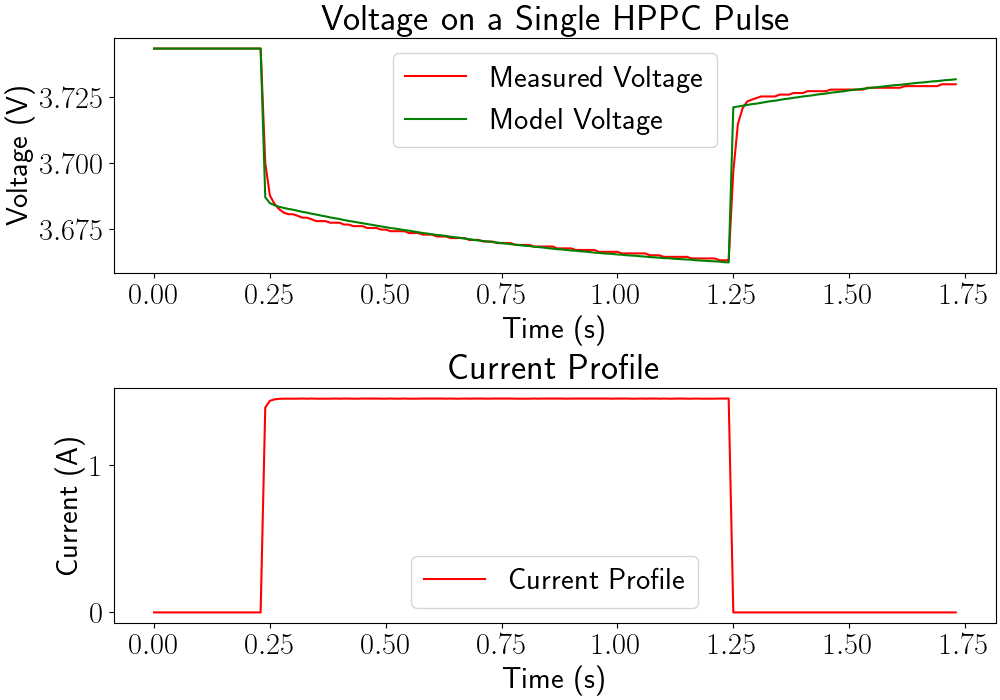
\includegraphics[width=0.6\linewidth]{figures/hppc-pulse.png}
    \caption{One of the sample HPPC (Hybrid Pulse Power Characterization) pulses we used for parameter finding. We want to model the output voltage $V(t)$ given a current input profile $I(t)$. Each sample is characterised at a specific state of charge $s$, state of health $h$ and temperature $T$, this one was taken at $s \approx 1$, $h \approx 1$ and $T = \SI{10}{\degreeCelsius}$.}
    \label{fig:hppc-pulse}
  \end{figure}

  Empirically, we know that a battery's voltage output looks roughly as given in \autoref{fig:hppc-pulse}, which is part of a standardised cycle characterisation procedure taking the battery from ``fully charged'' ($s=1$) to ``completely empty'' ($s=0$). Data is due to \cite{panasonicnums}.
  As one can see from the voltage curve, the battery exerts a ``time-relaxation'' behaviour on high-frequency changes in the current.
  One way of modelling this is through an RC circuit, confer \autoref{fig:ecm}: the parallel circuit of $R_1$ and $C_1$ is responsible for an exponential-looking behaviour in the voltage curve given (near-)jumps in the current.
  Normally, RC circuits also
  Additional ohmic impedance is modelled through $R_0$.
  The ``heart'' of the equivalent circuit model is the open-circuit voltage $V_{OC}$ which behaves like a voltage source but strongly depends on parameters $s$, $h$ and $T$.
  We modelled it accordingly, using a polynomial ansatz including cross-terms $$V_{OC}(s, h, T) = c_1 s + c_2 h + c_3 T + c_4 sh + c_5 sT + c_6 hT + c_7 shT + \mathcal{O}(s^2, h^2, T^2, ...)\,,$$
  and similar polynomials are chosen for $R_0$, $R_1$ and $C_1$, completing the model.

  \begin{figure}[H]
    \centering
    \inputtikz{ecm-model}
    \caption{
      The Thevenin equivalent circuit model (ECM) with parameters $R_0 \in \R^+$, $R_1 \in \R^+$ and $C_1 \in \R^+$ and $V_{\rm OC} \in \R^+$ the \textit{open circuit voltage} which behaves according to a function $V_{\rm OC}(s, h, T)$ dependent on $s$, $h$ and $T$.
    }
    \label{fig:ecm}
  \end{figure}

  Kirchhoff's law then tells us that the currents $I_{R1} \in \R$ and $I_{C1} \in \R$ add up to the total current $I = I_{R1} + I_{C1}$, and that the voltages $V_0 \in \R$, $V_1 \in \R$ and $V_{\rm OC}$ sum up to $V = V_0 + V_1 + V_{\rm OC}$.
  The capacitor behaves according to $I_{C1} = C_1 \frac{\dd V_1}{\ddt}$, while the resistors follow Ohm's law $V_0 = R_0 I$ and $V_1 = R_1 I_{R1}$.
  The resulting circuit then behaves approximately as a real Lithium-Ion battery would in many relevant situations.
  Let us consider an application of this model in an electric vehicle next.

  \subsection{Battery in an Electric Vehicle (EV)}
  In order to model a road network, let us first consider the definition of an undirected graph $G = (V_G, E)$. We take an undirected graph for simplicity, assuming that cars may go in arbitrary direction along each edge.
  \begin{definition}{Undirected Graph}{undirected-graph}
    A graph $G = (V_G, E)$ with vertices $V_G$ and edges $E \subseteq V_G \times V_G$ is undirected if and only if $(v_i, v_j) \in E \Rightarrow (v_j, v_i) \in E \quad \forall\; v_i, v_j \in V_G$.
  \end{definition}

  Modelling a vehicle on a road network requires a few more definitions.
  On a graph $(V_G, E)$ with edges $E = \{AB, AC, ...\} \subseteq V_G \times V_G$ and vertices $V_G = \{A, B, ...\}$, let
  $d_{AB} \in \R^+$ denote the distance between two vertices $A \in V_G$ and $B \in V_G$ (\textcolor{gray}{in meters}),
  $x = x_{AB} \in [0, d_{AB}]$ the progress (current location) on the route from vertex $A$ to $B$ (\textcolor{gray}{in meters}),
  $v := \frac{\ddx}{\ddt}$ denote the current velocity with
  $v_{\rm max, AB} \in \R^+$ the maximum allowed velocity on $AB$ (\textcolor{gray}{in meters per second}).
  Then let
  $T_{\rm env}(x) \in [-273.15, \infty)$ denote the temperature of the environment (\textcolor{gray}{in degrees Celsius}) at location $x$.
  Note that this graph-based approach to the problem does not require any more geometric information about the network than edge lengths $\{d_{ij}\}_{i,j}$, while it may of course be motivated by spherical coordinates on the earth.
  Consider for example \autoref{fig:graz-to-munich} or \autoref{fig:grannys-stations} for an actual route in Ireland.

  \begin{figure}[H]
    \centering
    \inputtikz{graz-to-munich}
    \caption{Exemplary route from Graz to Munich on a road network $(V_G, E)$, where edge weights correspond to distances in between the physical places represented by nodes.}
    \label{fig:graz-to-munich}
  \end{figure}

  The model of our car still lacks a component realising electrical into mechanical power (a motor), which we model very in a very ordinary fashion.
  Let $P \in \R$, $P := I \cdot V$ denote the (electrical) power the car draws from the battery (\textcolor{gray}{in Watts}) so $P > 0$ corresponds to discharging the battery.
  This power is to be realised into a mechanical component $P_{\rm motor} \in \R^+$ driving the car forwards, heating for the battery $P_{\rm heat} \in \R^+$, $P_{\rm heat} = c (T - T_{\rm env})$, with $c \in \R^+$ the heat conduction constant describing the relation between the heater and battery, and power dissipation $P_{\rm diss} \in \R^+$.
  While driving, $P = P_{\rm motor} + P_{\rm heat} + P_{\rm diss}$.
  The acceleration of the car $a \in \R$ (\textcolor{gray}{in meters per second squared}), where $a := \frac{\dd v}{\ddt} = \frac{\dd^2 x}{\ddt}$ is decomposed into $a_m \in \R$, which directly impacts $P_{\rm motor}(a_m)$, and the deceleration due to friction (air, etc.) $a_f(v) \in \R^-$, so that in total $a = a_m + a_f$.

  Most electric cars have a range from approximately 160 up to 650 km \parencite{range}, making route changes through charging stations a necessity for longer trips.
  The resulting routing problem we want to solve then inspires the following definitions of charging stations.
  On the graph $(V_G, E)$ there exists a set of EV charging stations $V_{\rm charge} \subseteq V_G$ where $P_{C,\rm charge}$ denotes the possible charging power (\textcolor{gray}{in Watts}) at the charging station vertex $C \in V_{\rm charge}$ with $K_C \in \R^+$ the occuring costs per energy unit (\textcolor{gray}{in Euros per Watt second}) and $t_C \in \R^+$ the charging time per charging station $B$ (\textcolor{gray}{in seconds})\footnote{
    Charging station \& street data was obtained from \href{https://osm.org/}{OpenStreetMap} and subsequently invoking
    \texttt{osmfilter england-latest.o5m \-\-keep="amenity=charging\_station"}.
    Daily dumps of OSM's public map data were obtained from \url{https://download.geofabrik.de/}.
  }.

  \subsection{Battery Aging}
  A central aspect considered in our project was to study the effects of battery degredation, or aging. One possible model for this would be to express $Q_0$ in terms of the original capacity at the time of production $Q_{00}$ along with multiple degradation effects that we consider:
  \begin{equation*}
    \label{eq:cap}
    Q_0(t,c,s,I) = Q_{00} - \frac{F_{\rm acycle}(c)}{F_{\rm current}(I)} - F_{\rm cal} \quad \in [0, Q_{00}]\,.
  \end{equation*}
  By $F_{\rm acycle}(c)$ we denote the \textit{Current Agnostic Cycle Degradation Factor} models cycle aging at a single current.
  Also $F_{\rm current}(I)$ represents the \textit{Current Scaling Factor}, a value $0 < F_{\rm current} \leq 1$ that incorporates behaviour where higher currents are worse for cycle aging \parencite{csfpaper}.
  Finally, $F_{\rm cal}(s,t)$, the \textit{Calendar Degradation Factor}, ages the battery over time and accounts for suboptimal storage in terms of state of charge.

  The state of health is then given by
  $$h = \frac{Q_0}{Q_{00}} = 1 - \frac{F_{\rm acycle}(c) + F_{\rm cal} F_{\rm current}(I)}{F_{\rm current}(I) Q_{00}} \quad \in [0, 1]\,.$$

  \begin{figure}[H]
    \centering
    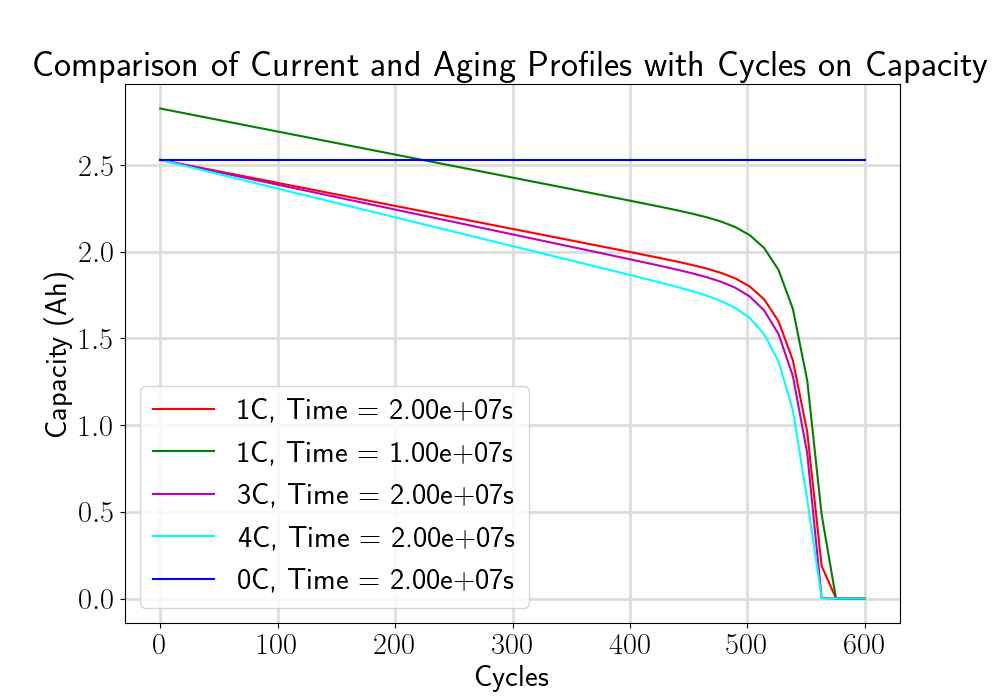
\includegraphics[width=0.7\linewidth]{figures/aging.png}
    \caption{Aging}
    \label{fig:aging}
  \end{figure}

  Using the car and road network models introduced above, in general terms the problem may be stated as follows:

  \subsection{A Variational Optimisation Problem}
  Given source and destination vertices $A, Z \in V_G$ on the graph $(V_G, E)$, \textbf{which connected set of edges} $E_R \subseteq E$ connecting $A$ to $Z$, set of visited \textbf{charging stations} $V_C \subseteq V_{\rm charge}$ along $E_R$ and \textbf{charging times} $\{t_C\}_{C \in V_C}$ visited on the route $E_R$, and \textbf{driving behaviour} $a_m(x, v, t, s, h, T_{\rm env}, ...),\, a_m \in \cC^1(\P)$ with $\P$ the parameter space, \textbf{minimises}
  \begin{enumerate}
    \item the total travel time $t_{\rm total} := \int_{V_R} \frac{1}{v} \,\ddx + \sum_{C \in V_C} t_C$,
    \item the total cost of travel $K := \sum_{C \in V_C} P_{C, \rm charge} t_{C} K_C$,
    \item or $-N$ where $N$ is the highest possible number of repetitions (commutes from $A$ to $Z$) with the same battery (requiring $h > 0$). \label{minoption:aging}
  \end{enumerate}
  In other words, we aim to minimise the functional $F \in \cC(\P)^*, F: \cC(\P) \mapsto \R$ where either $F[a_m] = t_{\rm total}$, $F[a_m] = K$ or $F[a_m] = -N$.

  % \subsection{Notes}
  % \begin{itemize}
  %   % \item
  %   \item Thanks to Nicholas and Zella, we have $R_0$, $R_1$, $C_1$ as functions of $s$, $T$ (and possibly $h$ in the future).
  % \end{itemize}

  % \subsection{Simplifications}
  % Endless possibilities, such as
  % \begin{itemize}
  %   \item $V_G = \{A, B\}$ and $E = \{AB\}$ with some $d_{AB}$ and $v_{\rm max, AB} = \infty$ and $V_C = \{\}$, so only looking at the minimisation of $t_{\rm total}$.
  %   \item $P_{\rm heat} = 0$.
  %   \item $T = T_{\rm env} = \rm const.$ and therefore $P_{\rm heat} = 0$.
  %   \item $P_{\rm diss} = 0$.
  %   \item $a_f = 0$.
  %   \item $h = 1$.
  %   \item $s = \rm const$.
  %   \item etc.
  % \end{itemize}
  % and many more simplifications are possible, which ones do we choose?

  \begin{figure}[H]
    \centering
    \inputtikz{battery-model-overview}
    \caption{Overview}
    \label{fig:model-overview}
  \end{figure}

  \section{Numerical Simulation of a Car}
  For simplification, we neglected temperature changes in the environment and a respective battery heating strategy $P_{\rm heat}(x, v, t, s, h, T_{\rm env}, ...)$, $P_{\rm heat} \in \cC(\P)$.

  \subsection{Finding ECM Parameters}
  \begin{figure}[H]
    \captionsetup[subfigure]{justification=centering}
    \centering
    \subfloat[Fit of $R_0$ as a function of the SOC ($s$).]{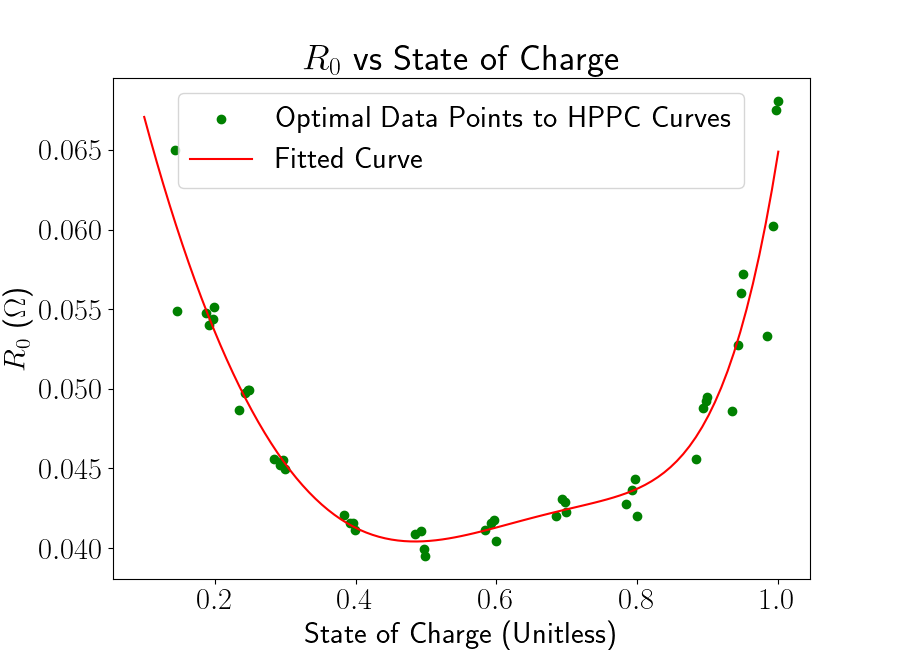
\includegraphics[width=.5\linewidth]{figures/r0fit.png}}\hfill
    \subfloat[Fit of $R_1$ as a function of the SOC ($s$).]{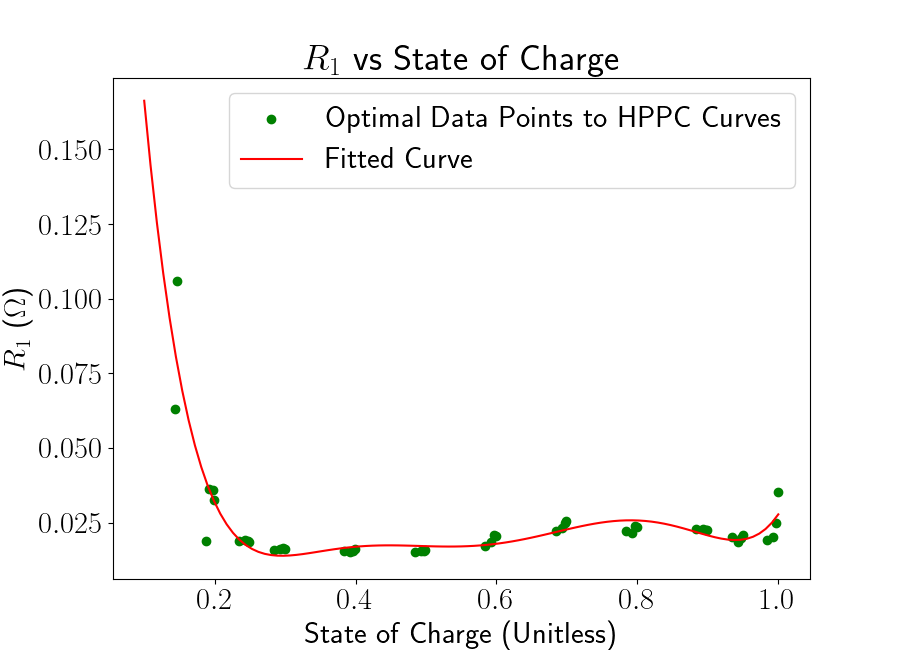
\includegraphics[width=.5\linewidth]{figures/r1fit.png}}\par
  \end{figure}

  \subsection{Forward Euler Simulation}

  \begin{figure}[H]
    \centering
    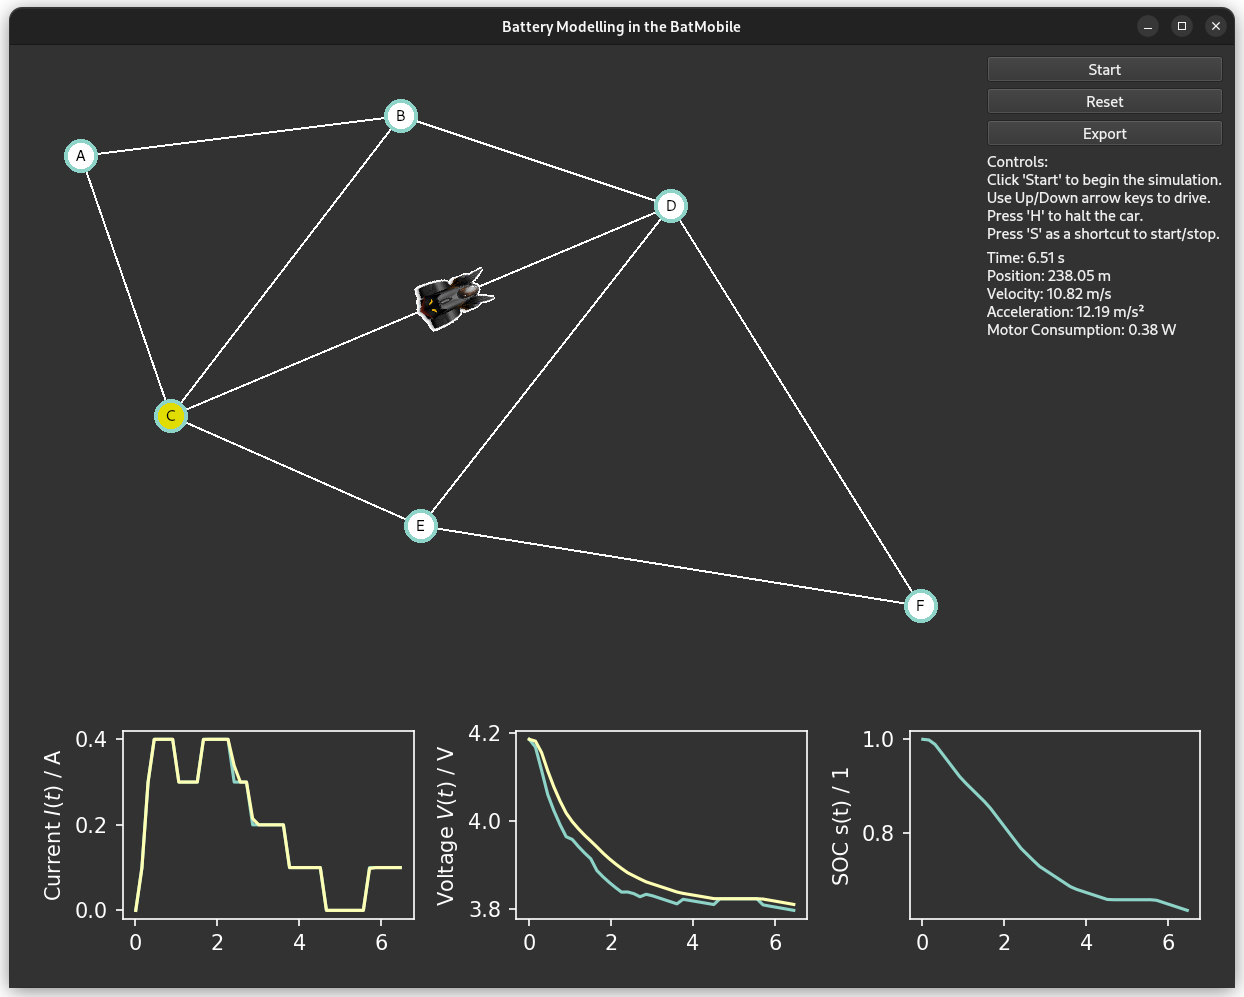
\includegraphics[width=0.8\linewidth]{figures/screenshot.png}
    \caption{User Interface}
    \label{fig:user-interface}
  \end{figure}

  \section{Metropolis-Hastings and A-Star}
  \subsection{Shortest Path Finding}
  The graph data was retrieved using OSMNX \parencite{osmnx} which itself is built on NetworkX \parencite{networkx}.

  \subsection{Monte-Carlo Optimisation}
  Optimise a large problem (huge state-space). Metric: Time! Could be anything.
  $\Rightarrow$ Use Monte-Carlo Markov Chain Methods!
  Slightly perturb the route using a specific alteration technique.
  Metropolis-Hastings updates the state (route) based on $$p_{\rm accept} = \min\left(1, \e^{-\beta (T_{\rm next} - T_{\rm current})}\right)\,, \quad \text{ with } \beta \in \R^+ \text{ a transition factor} \,.$$
  Does a full numerical simulation of the drive. Stop to charge?
  Explore the state-space to some extent, and return the best route!
  Larger scales / maps (e.g. England) are not a problem!

  \begin{minted}{python}
newEnergy = self.measureRoute(newRoute) if newRoute not in self.testedRoutes else self.testedRoutes[newRoute]
delta = newEnergy - self.testedRoutes[self.route]
acceptanceProbability = min(1, math.exp(-delta / self.temperature))
if random.random() < acceptanceProbability:
    self.route = newRoute
    print(f"Accepted new route {newRoute} with delta: {delta:.2f}. Total: {self.testedRoutes[newRoute]:.2f}.")
else:
    print(f"Rejected route {newRoute} with delta: {delta:.2f}.")
  \end{minted}

  \subsection{Special Case: Granny's House}
  \begin{figure}[H]
    \centering
    \inputtikz{grannys-house}
    \caption{The exemplary problem ``Granny's House'', a special case of Problem (TODO).}
    \label{fig:grannys-idealised-problem-setting}
  \end{figure}

  \begin{figure}[H]
    \centering
    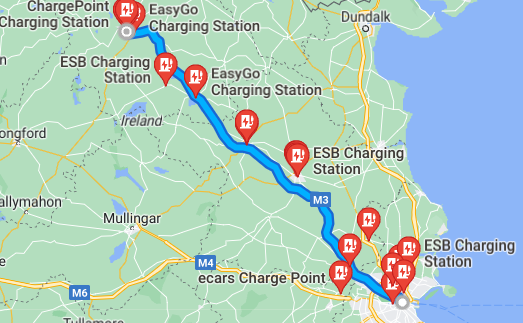
\includegraphics[width=0.4\linewidth]{figures/grannys-stations.png}
    \caption{Route in Ireland}
    \label{fig:grannys-stations}
  \end{figure}

  \subsection{Routing in Jericho}
  \begin{figure}[H]
    \centering
    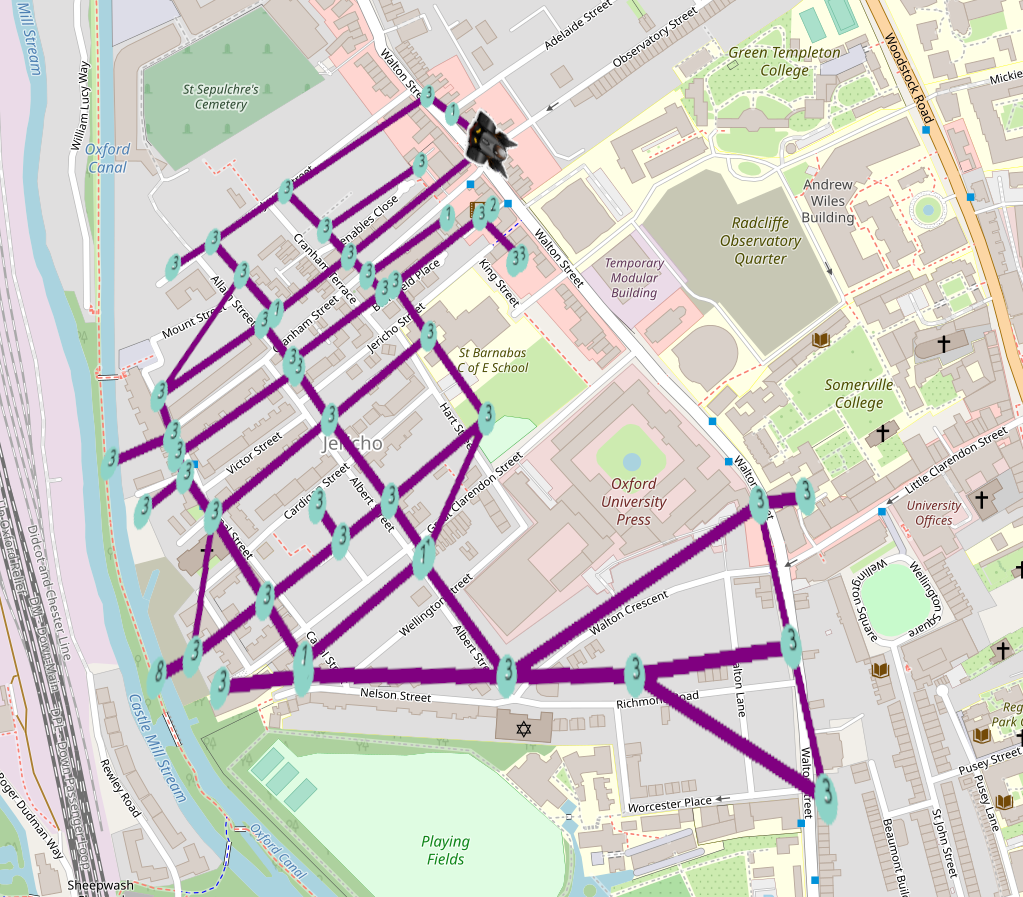
\includegraphics[width=0.6\linewidth]{figures/jericho.png}
    \caption{Overlay of the routing graph on a map of Jericho \parencite{osm}, without adjusting for the Merkator projection, which leads to a slightly skewed appearance. The underlying data is exactly the same.}
  \end{figure}

  \begin{figure}[H]
    \captionsetup[subfigure]{justification=centering}
    \centering
    \subfloat[Route 1.]{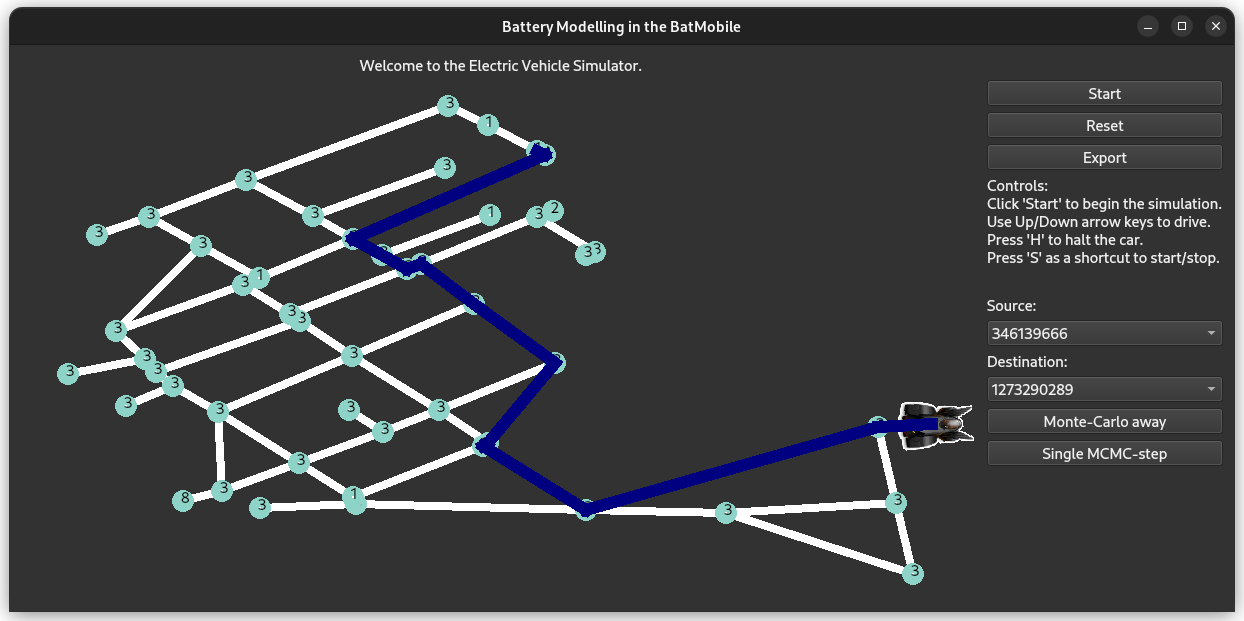
\includegraphics[width=.5\linewidth]{figures/route1.png}}\hfill
    \subfloat[Route 2.]{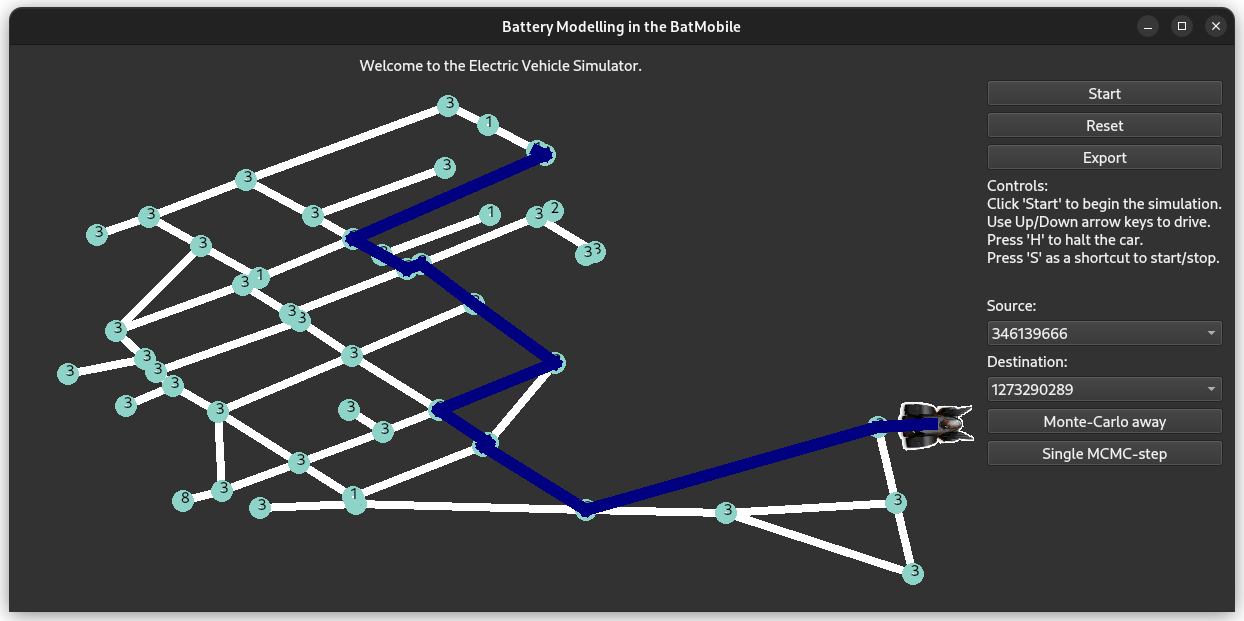
\includegraphics[width=.5\linewidth]{figures/route2.png}}\par
    \vspace{0.5cm}
    \subfloat[Route 3.]{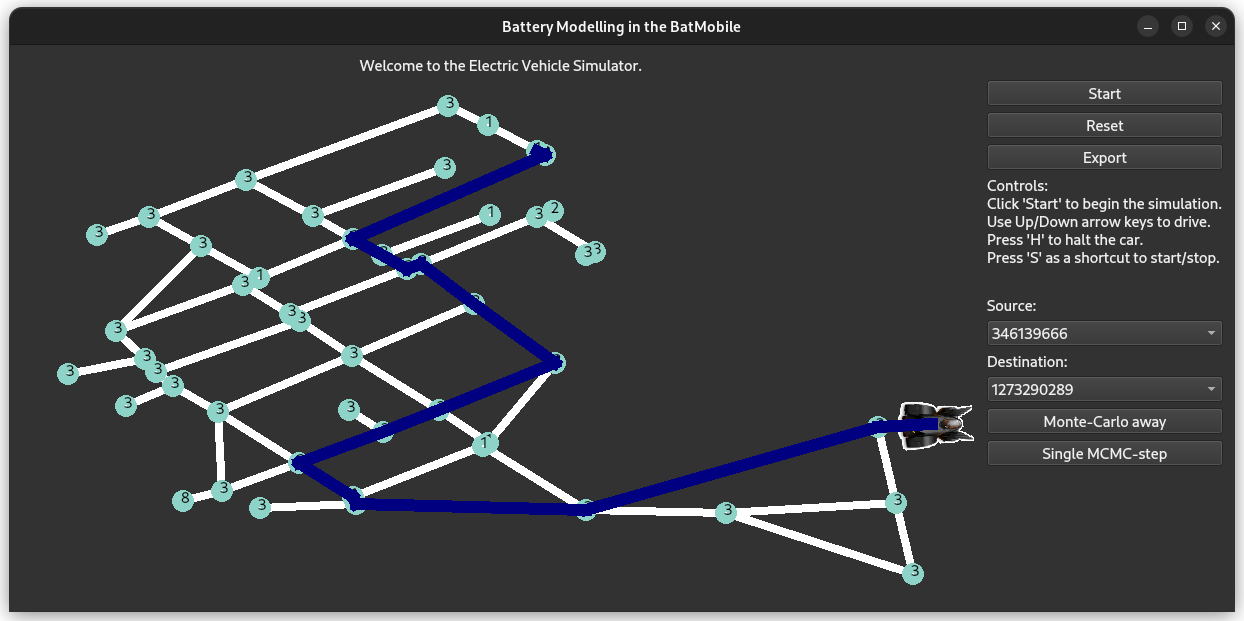
\includegraphics[width=.5\linewidth]{figures/route3.png}}\hfill
    \subfloat[Route 4.]{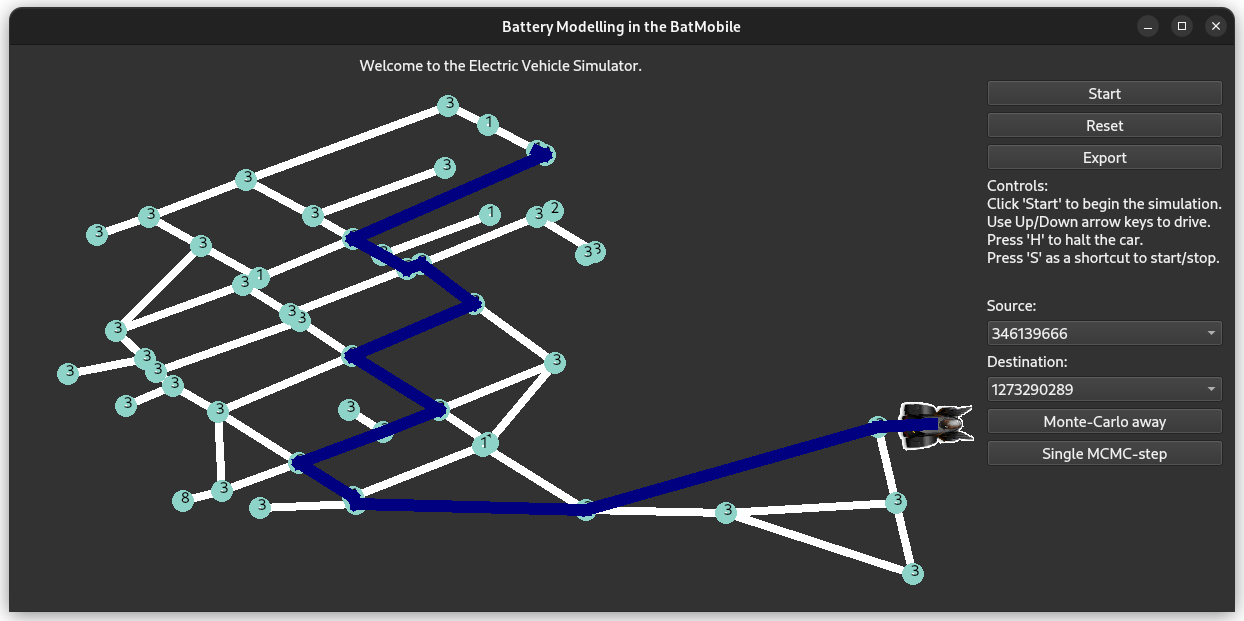
\includegraphics[width=.5\linewidth]{figures/route4.png}}\par
    \caption{Routes}
  \end{figure}

  \section{Conclusion}

  \pagebreak
  \printbibliography

  \pagebreak
  \appendix
  % \section{Simulation Code}
  % \inputminted{python}{../simulator/optimiser.py}

  \section{Code Structure and Setup}
  The code can be found on GitHub, namely in \href{https://github.com/MrP01/BatteryModelling}{this repository}.
  To use and sustain a Python virtual environment, install
  \href{https://python-poetry.org/}{poetry}, which works with the
  \texttt{pyproject.toml} file. After installing poetry (and subsequently
  after pulling, each time), run \\
  \mintinline{bash}{poetry install} \\
  in the project folder. To install PyBamm as well (which has $\mathcal{O}(\frac{1}{\epsilon})$ number of dependencies), run \\
  \mintinline{bash}{poetry install --with=pybamm} \\
  instead or additionally. This sadly requires Python 3.8 based on a
  pybamm restriction. Without pybamm, 3.11 should be fine too.

  Having all dependencies installed, the main interface may be launched up
  by executing \\
  \mintinline{bash}{python3 main.py} \\
  which starts a graphical user interface (with looks depending on your
  operating system). Note that you may need to install some Qt6 dependencies.

  The relevant code structure is:

  \begin{itemize}
    \tightlist
    \item
          The folder \texttt{simulator/} is responsible for the (numerical)
          simulation itself, which may be invoked without any interface at all.

          \begin{itemize}
            \tightlist
            \item
                  \texttt{simulation.py} features the Simulation class with an
                  \texttt{iterate()} method that represents a numerical integration
                  step in time by an amount of \texttt{dt}.
            \item
                  \texttt{batgraph.py} exports a class \texttt{BatGraph} that
                  represents a graph (a tuple of sets of edges and vertices) that the
                  car will drive on.
            \item
                  \texttt{batmobile.py} contains the \texttt{BatMobile} class that
                  represents our battery mobile i.e.~car. \textbf{Much of the
                    simulation takes place in this file!}
            \item
                  \texttt{battery.py} is the central file for our battery modelling
                  project, which exports a \texttt{Battery} class, also featuring an
                  \texttt{iterate()} method. \textbf{Most of the battery simulation
                    takes place in this file!}
            \item
                  \texttt{optimiser.py} takes care of the optimisation part of the routing problem. It implements the Metropolis-Hastings (Monte-Carlo Markov Chain) method and defines the graph perturbations.
          \end{itemize}
    \item
          The interface code is contained within the \texttt{interface/} folder.

          \begin{itemize}
            \tightlist
            \item
                  \texttt{mainwindow.py} defines the general layout and actions in the
                  user interface.
            \item
                  \texttt{batmap.py} exports the central widget that renders /
                  animates the BatMobile car on the BatGraph.
            \item
                  \texttt{graphs.py} handles the connection of the interface and
                  (live) plots. The plots are handled by \texttt{matplotlib} and are
                  very intuitive to use, further almost all commands are the same as
                  they are in MatLab.
          \end{itemize}
    \item
          \texttt{main.py} creates a \texttt{MainWindow} and runs the simulator
          GUI.
  \end{itemize}
\end{document}
